\section{k-NN}
The k-nearest neighbor (kNN) algorithm is a nonparametic classification algorithm. It is been known for its simplicity and accuracy.
It is a supervised learning algorithm, that means, that a labled traning dataset is been used to train the model and afterwards a class of unlabled data can be classified.
It is a "lazy learning" algorithm that means it does not achieve generalizations. The entire traningset is being used for traning.
When a new unlabled data is presented into the dataset, the k-NN algorithm determines in wich class the unlabled data should go by determining the wich classes the neighboring belong to.
Outlier detection is a binary classification problem. That means, that the considered neighbors for a new tuple, only can be inliers or outliers. 
If the 


There are two operations calculated, when new data is presented to the model:
\citep[p.1256 pp.]{9065747}


$K$ is the number of neighbors that would be considered for classifying a new unlabled tuple. 
Even though this classifier is simple, the value of ‘K’ plays an important role in classifying the unlabeled data.
$K$ is an hyperparameter, that means it is an external configuration variable that need be determined befor the process begins.
It is task of hyperparamatic tuning to find a optimal number of $k$. 
You have to consider the bias-variance-trade of when you choose the optimal $K$. 
The smaller $K$ is, the more likley it is that the model suffers from overfitting, leading to higher variance and lower bias.
The resulting decision boundaries will be complex and fragmented.
The lager $K$ ist, the more likley it is, that the model suffers from underfitting, leading to smaller variance and lagrer bias.
The resulting decision boundaries maybe missing local patterns.
It is advised to choose a odd-number $K$, otherwiseat at an even classification the model could fail.  


To determine the nearest neighbor, you need to calculate the distance between the new tuple and the neighbors. 
In classical k-NN, you use the Euclidean distance. 
By using the Euclidean-distance , k-NN is not affine equivariant.
Non-uniforly changes in the scale changes the distance landscap and thus leading to different set of nearest neighbors.
Resulting in different classifications. 


k-NN has many advantages. Its results are easy to understand and interpret.
The algorithm stays efficient with large traning sets eventhough it is invfluence by the curse of dimensional
There is no need for complex mathematical calculations, making it user-friendly.
Its is a non-paramatic model, that does not require any assumptions about the underlying distribution od the dataset.
That makes it flexible for complex datasets.


Some disadvantage of k-NN might be: the computational complexity. 
For a classification the model requires to store the entire dataset. Especially for large datasets, that could lead to slow prediction time. 
Moreover, storing the entire dataset is memory-intensive.
Because of the dependence of distance measurments, noisy data can influence the accurarcy negatively.
Chosing $K$ is vital for the models results. Through hyperparamatric tuning, one has to optimize the model. 

\begin{figure}[h] 
    \centering
    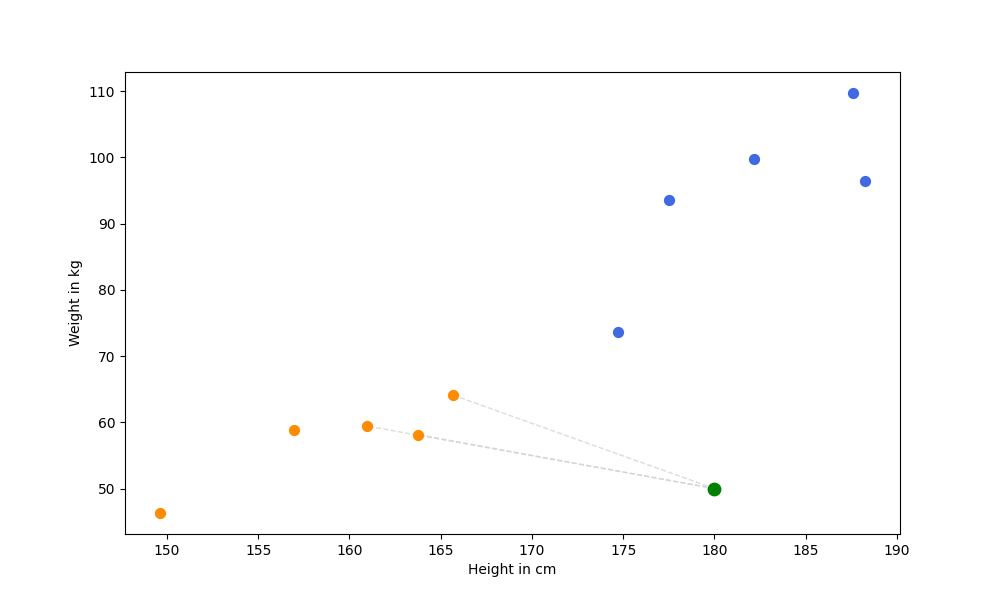
\includegraphics[width=1\linewidth]{Images/kNN/k-NN.png}
    \caption{grapfical depiction of k-NN algorithm}
    \label{fig:my_example}
\end{figure}

\textcolor{red}{\citep{yang2023outlier} for further information}


\newpage
\textcolor{green}
{The k-nearest-neighbor global unsupervised anomaly detection algorithm is a straightforward
way for detecting anomalies and not to be confused with k-nearest neighbor classification. As
the name already implies, it focuses on global anomalies and is not able to detect local anoma-
lies. First, for every record in the dataset, the k-nearest-neighbors have to be found. Then, an
anomaly score is computed using these neighbors, whereas two possibilities have been pro-
posed: Either the distance to the k th-nearest-neighbor is used (a single one) [41] or the average
distance to all of the k-nearest-neighbors [42] is computed. In the following, we refer to the
first method as kth-NN and the latter as k-NN. In practical applications, the k-NN method is
often preferred [13, 19]. However, the absolute value of the score depends very much on the
dataset itself, the number of dimensions, and on normalization. As a result, it is in practice not
easy to select an appropriate threshold, if required.
The choice of the parameter k is of course important for the results. If it is chosen too low,
the density estimation for the records might be not reliable. On the other hand, if it is too large,
density estimation may be too coarse. As a rule of thumb, k should be in the range 10 < k < 50.
In classification, it is possible to determine a suitable k, for example by using cross-validation.
Unfortunately, there is no such technique in unsupervised anomaly detection due to missing
labels. For that reason, we use later in the evaluation many different values for k and average in
order to get a fair evaluation when comparing algorithms.
In Fig 4 we exemplary illustrate how the result of an unsupervised anomaly detection algo-
rithm (here: k-NN with k = 10) can be visualized. The plot was generated using a simple, artifi-
cially generated two-dimensional dataset with four Gaussian clusters and uniformly sampled
anomalies. After applying the global k-NN, the outlier scores are visualized by the bubble-size
of the corresponding instance. The color indicates the label, whereas anomalies are red. It can
be seen, that k-NN cannot detect the anomalies close to the clusters well and assign small
scores \citep[p.8+9]{goldstein2016comparative}}



